\documentclass[11pt]{article}
\usepackage{amssymb,amsmath}


\usepackage{enumitem}
\setlist[enumerate, 1]{label=\arabic*., ref = \arabic*}
\setlist[enumerate, 2]{label=\alph*., ref=\theenumi.\alph*}
\setlist[enumerate, 3]{label=(\alph*), ref=\theenumii.(\alph*)}

%\setenumerate[1]{label=(\Alph*)}
%\setenumerate[2]{label=(\Alph)}

\numberwithin{equation}{enumi}
\usepackage[toc, page]{appendix}
\usepackage[makeroom]{cancel}
\usepackage{physics}
\usepackage{soul}
\usepackage{fullpage,graphicx,psfrag}
\usepackage{amssymb,amsmath,amsthm,amsfonts,mathtools, verbatim}
\usepackage[small,bf]{caption}
\usepackage{tcolorbox,tikz,color,graphics,subcaption}
\usetikzlibrary{decorations.pathreplacing,calc}
\usepackage{tcolorbox}

\pagestyle{empty}

%%%%%%%%%%%%%% Swati's stuff
\usepackage[noabbrev,capitalize]{cleveref} 
\crefname{eq}{Equation}{Equations}
\crefname{optn}{Problem}{Problems}
\crefname{defn}{Definition}{Definitions}
\crefname{app}{Appendix}{Appendices}
\crefname{ineq}{Inequality}{Inequalities}
\creflabelformat{ineq}{(#2{\upshape #1}#3)} % adjust position of parentheses so that the hyperlink box is either outside or inside of parentheses.
\crefname{subsection}{Section}{Sections} % change the second/third arguments if you want to change how subsections are referenced
\crefname{subsubsection}{Section}{Sections}
\crefname{remark}{Remark}{Remarks}
\crefname{lemma}{Lemma}{Lemmas}
%\crefname{figure}{Figure}{Figures}

\input defs.tex
\begin{document}

\vspace{-20mm}

\setlength{\fboxrule}{.5mm}\setlength{\fboxsep}{1.2mm}
\newlength{\boxlength}\setlength{\boxlength}{\textwidth}
\addtolength{\boxlength}{-4mm}
\begin{center}\framebox{\parbox{\boxlength}{\bf
 Machine Learning \hfill Homework 2\\
CSE 546 Fall 2017 \hfill  October 21, 2017 \\
Swati Padmanabhan}}\end{center}
\vspace{1mm}
NOTE: Collaborated with Robbie Weber. 
\begin{enumerate}
	\item Least Squares. Dimensions: $x \in \reals^d$, $y \in \reals^n$, $X \in \reals^{n \times d}$ and $\varepsilon \in \reals^n$. Therefore, $X X^T \in \reals^{n \times n}$, $X^T X \in \reals^{d \times d}$. 
	\begin{enumerate}
		\item The given expression is $\hat{w} = (X^T X)^{-1} X^T y$. Substitute the given expression for $y$, 
			 \[\hat{w} = (X^T X)^{-1} X^T (X w^* + \varepsilon) = w^* + (X^T X)^{-1} X^T \varepsilon . \numberthis\label{what}\]
		 
		\item Define \[ U =  (X^T X)^{-1} X^T .\numberthis\label[defn]{U}\] Let $U_i$ represent the ith row of $U$. Then from \cref{what}:
			\begin{align*}
				 \E_\varepsilon \hat{w} &= w^* +  [\E_{\varepsilon} U_i^T \varepsilon] \\
													&= w^*, \numberthis\label{exp-what}
			\end{align*}
			where the last equality is because $\varepsilon_i \sim \mathcal{N}(0, \sigma^2)$ for all $i = 1, \dotsc, n$, so $\E_{\varepsilon} U_i^T \varepsilon = \sum_{j = 1}^n U_{ij} \E_{\varepsilon_j} \varepsilon_j = 0$. Again from \cref{what} 
			\begin{align*}
				 \E_\varepsilon \norm{\hat{w} - w^*}_2^2 &= \E_\varepsilon\norm{U \varepsilon}_2^2\\
																	&= \E \varepsilon^T U^T U \varepsilon\\
																	&= \E \Tr  \varepsilon^T U^T U \varepsilon\\
																	&= \E \Tr \varepsilon \varepsilon^T U^T U \\
																	&=  \Tr \E \varepsilon\varepsilon^T U^T U \\
																	 &= \Tr \sigma^2 U^T U \\
																	 &= \sigma^2 \Tr U^T U \\
																	 &= \sigma^2 \Tr (X^T X)^{-1}. \numberthis\label{exp-what-wstar-normsqr}
			\end{align*}
		\item For the first expectation: 
			\begin{align*}
				\E_{\teps} (\tilde{y}) &= \E_{\teps} (X w^* + \teps) \\
									 &= X w^* + \E_{\teps} \teps = X w^*. \numberthis\label{exp-ty}
			\end{align*}
			where the last expression follows from substituting $\hat{w}$ from \cref{what} and \cref{U}. Next, to make calculations simpler, we observe that:  
			\begin{align*}
				\tilde{y}_i - x_i^T \hat{w} &= (x_i^T w^* + \teps_i) - x_i^T \hat{w} \\
											 &= x_i^T ( w^* - \hat{w}) + \teps_i \\
											 &= -x_i^T U \varepsilon	 + \teps_i.\\
			 	\therefore \sum_{i = 1}^n (\tilde{y}_i - x_i^T \hat{w})^2 &= \sum_{i = 1}^n (-x_i^T U \varepsilon	 + \teps_i)^2 \\
			 																&=\norm{ X U \varepsilon - \teps}_2^2.
			\end{align*}
			We first compute the inner expectation. Let $M =  XU$. 
			\begin{align*}
				\E_{\varepsilon}  \sum_{i = 1}^n (\tilde{y}_i - x_i^T \hat{w})^2 &= \E_{\varepsilon} \norm{ X U \varepsilon - \teps}_2^2\\
																				&= \E_{\varepsilon}  \norm{M \varepsilon}_2^2 + \E_{\varepsilon}\norm{\teps}_2^2 \\
																			    &=  \E_{\varepsilon} \varepsilon^T M^T M \varepsilon + \norm{\teps}_2^2\\
																			    &= \E_{\varepsilon} \Tr \varepsilon^T M^T M \varepsilon +  \norm{\teps}_2^2\\
																			   &=  \Tr \E_{\varepsilon}  M^T M \varepsilon \varepsilon^T +  \norm{\teps}_2^2\\
																			   &= \Tr M^T M \sigma^2 I + \norm{\teps}_2^2\\
																			   &= \Tr ((X^T X)^{-1} X^T  X (X^T X)^{-1} X^T X) \sigma^2  + \norm{\teps}_2^2\\
																			   &= n \sigma^2 + \norm{\teps}_2^2.
			\end{align*}
			Taking outer expectation: 
			\begin{align*}
				\E_{\teps} \E_{\varepsilon}\frac{1}{n} \sum_{i = 1}^n (\tilde{y}_i - x_i^T \hat{w})^2 &= \E_{\teps}  \frac{1}{n} (n \sigma^2 + \norm{\teps}_2^2) \\
																			       &= \sigma^2 + \frac{1}{n}\E_{\teps} \sum_{i = 1}^n \teps_i^2 \\
																			       &= 2\sigma^2. \numberthis\label{exp-crazy-var}
			\end{align*}
			
			
	\end{enumerate}
	
	\item 
	\begin{enumerate}
		\item Set $z_i = \ones_{(f(x_i) \neq y_i)}$. Then we have by Hoeffding's inequality, 
		\[ \Prob \left( | \hat{L}(\tilde{f}) - L(\tilde{f}) | \leq A \right) \geq 1  - 2\exp( - 2 N A^2).\] Set the RHS to $1 - \delta$. This gives \[ A= \sqrt{\frac{1}{2N} \log \left( \frac{2}{\delta} \right)}.\] 
		\item 	Unfortunately yes. The same confidence interval holds, since there was nothing inherently about $f$ or $\tilde{f}$ that was used to compute the conjfidence interval. Just the fact that the empirical loss is computed by averaging over $N$ samples. 
		\item Ah, okay, this one is better. The proposed function $\hat{f}$ is, by definition, the one that brings the empirical loss closer to the true loss. So yes, the confidence interval \emph{is} changed!
		\item 
	\end{enumerate}
	
	\item 
 \begin{figure}[h!]
  \centering
  \begin{subfigure}[b]{0.32\linewidth}
    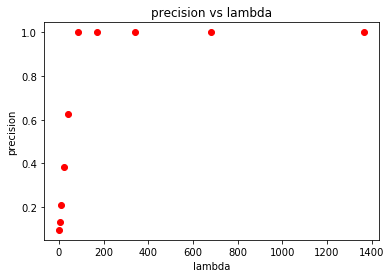
\includegraphics[width=\linewidth]{Problem3/prec-lam.png}
  \end{subfigure}
  \begin{subfigure}[b]{0.32\linewidth}
    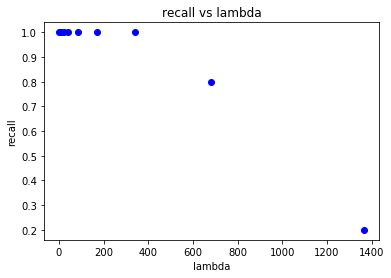
\includegraphics[width=\linewidth]{Problem3/rec-lam.png}
  \end{subfigure}
  \caption{Precision and Recall Curves.}
  \label{datasets}
\end{figure}
	The optimal $\lambda$ for perfect precision and recall is $400$. As $\lambda$ increases, we are forcing far too many elements to become zero (more than are actually zero). That's why the number of \emph{correct} non-zeros decreases (which is exactly recall). The precision, on the other hand, increases because the elements being set to zero are actually the ones that are zero. On synthetic data, this algorithm runs fast and is able to recover the zero patterns perfectly and get very good results on the non-zeros (signs are correct, values are very close to true ones). 
		
		\item 
\begin{figure}[h!]
  \centering
  \begin{subfigure}[b]{0.5\linewidth}
    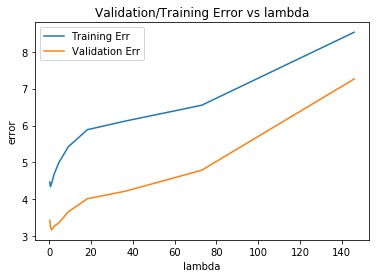
\includegraphics[width=\linewidth]{Problem4/train-val-err.png}
  \end{subfigure}
  \caption{Training and Validation Errors.}
  \label{datasets}
\end{figure}

	My best $\lambda$ is $4.5$ and the mean squared test error is $6.4$. 
	

	\item Using chain rule and some basic algebra: 
	\[ \nabla_w J(w, b) = \frac{1}{n} \sum_{i = 1}^n \frac{\exp(- y_i (b+ x_i^T w))}{1 + \exp(-y_i(b+x_i^T w))} (-y_i x_i) + 2\lambda w.\] Simplifying in terms of $\mu$, this equals \[ \frac{1}{n}\sum_{i = 1}^n (\mu_i(w, b) -1) y_i x_i + 2\lambda w.\] 
		
\end{enumerate}
\newpage
\nocite{*}
\end{document}

